\chapter*{Theory}

The small-scale structure of the Universe offers an avenue to test the nature of dark matter. The Lyman-alpha forest 1D power spectrum (P1D) can quantify the clustering of matter on small scales, $k \in [1, 10]~h~\mathrm{Mpc}^{-1}$, and thus constrain the properties of dark matter. The smallest scale that can be probed by this technique is set by the spectrograph resolution. The Spec-S5 will adopt the same spectrograph as DESI, which corresponds to a sensitivity to the matter power at $k\approx 1~h~\mathrm{Mpc}^{-1}$ at $z \sim 3.0$. Unless the dark matter leaves dramatic signatures on the matter power spectrum at these scales, the Spec-S5 Lyman-alpha forest P1D may not be able to definitely rule out or confirm the cold dark matter paradigm. However, a strong measurement of the amplitude and the slope of the matter power spectrum at $k \approx 1~h~\mathrm{Mpc}^{-1}$ could serve as an anchor point for other probes that are sensitive to smaller scales ($k\sim 10-100~h~\mathrm{Mpc}^{-1}$). In this white paper, we investigate the constraining power of the Spec-S5 Lyman-alpha forest P1D on the amplitude and slope of the matter power spectrum at $k \approx 1~h~\mathrm{Mpc}^{-1}$. We forecast the precision on these two parameters by studying the performance of this measurement in two redshift bins (rather than a single bin at $z_\star=3.0$).

\begin{figure}
    \centering
    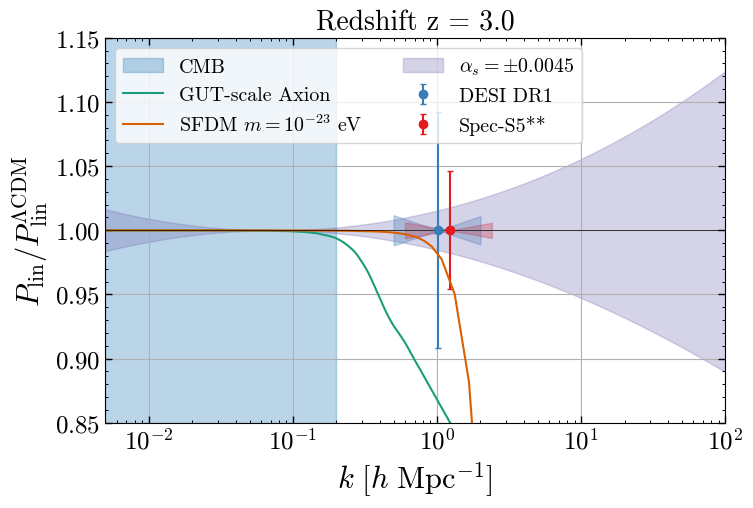
\includegraphics[width=0.7\linewidth]{farfield/plinear_lya.png}
    \caption{Linear matter power}
    \label{fig:plinlya}
\end{figure}

Figure \ref{fig:plinlya} shows the precision of DESI DR1 measurements on the amplitude and slope of the linear matter power spectrum at $k=1~h~\mathrm{Mpc}^{-1}$. The scales that are probed by CMB are shaded blue. We demonstrate two different dark matter models: (1) a GUT-scale Axion showing a strong deviation from the CDM, and (2) a scalar field dark matter model with a mass of $10^{-23}~\mathrm{eV}$ that cannot be constrained with DESI DR1 P1D measurements. In this same plot, we added a preliminary forecast for the Spec-S5 P1D measurement of the amplitude and slope of the matter power spectrum at the same scale but shifted for clarity. This is, so far, simply a factor-of-two improvement over the DESI DR1 measurement, but we are currently working to improve this forecast.

This factor-of-two forecast is based on an exercise in which we take the DESI DR1 P1D measurement and rescale the covariance matrix by some factor. We first assumed that a future DESI DR3 measurement will improve the statistical covariance matrix by a factor of 4 (a factor of 2 more quasars and another factor of 2 for doubling the exposure time), while the systematics cannot be improved: $C_{DR3} = C^{stat}_{DR1}/4 + C^{syst}_{DR1}$. Then, we assumed the Spec-S5 will further improve the statistical covariance matrix by a factor of 10, while the systematics cannot be improved: $C_{S5} = C^{stat}_{DR3}/10 + C^{syst}_{DR1}$. This is a very preliminary treatment, and we want to improve it by generating mock QSO and LBG spectra for the Spec-S5 forecast. Then, we performed a single-parameter amplitude-only Fisher forecast, such that our model is $P_{model}=\alpha P_{smooth}$ and the forecasted error on $\alpha$ is $\sigma^{-2}_\alpha = (P_{smooth}^T C^{-1} P_{smooth})$. By comparing the relative improvement from DR1 to Spec-S5, we arrived at a factor of two improvement on the amplitude of the matter power spectrum at $k=1~h~\mathrm{Mpc}^{-1}$. We have worked on reproducing the DR1 inference pipeline on two fronts: (1) using the same emulator, and (2) using the same full likelihood. The full likelihood includes many contaminants and nuisance parameters, which can make it more computationally expensive. 

\begin{figure}
    \centering
    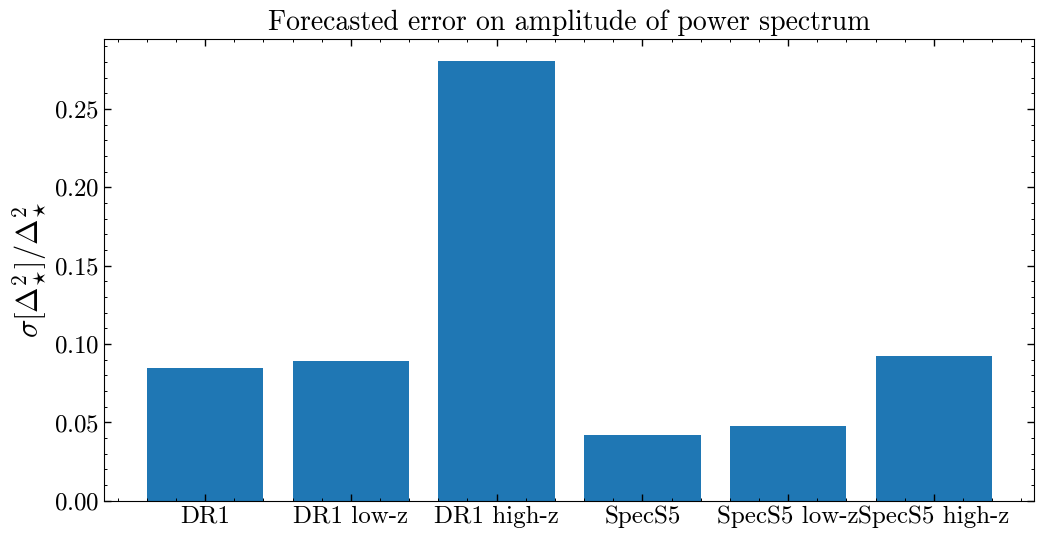
\includegraphics[width=0.7\linewidth]{farfield/single_parameter_forecast.png}
    \caption{Single parameter Fisher forecast}
    \label{fig:single_param_fore}
\end{figure}

Figure \ref{fig:single_param_fore} shows the outcome of this formalism. We also tested performing the same forecast in two redshift bins (low-$z$ is $z<3.5$, and high-$z$ is $z>3.5$) by splitting the covariance matrix into two. The improvement in the high-$z$ sample is more dramatic, since the low-$z$ sample saturates rapidly with systematics. Therefore, the return on investment at higher redshifts ($z\gtrsim 3.5$) is more significant. We then studied which systematics cost us the most constraining power. The uncertainty in DESI's spectrograph resolution is 1.5\% for DR1, and it may not improve substantially. Our preliminary forecast shows that the resolution is not a significant factor in the constraining power of Spec-S5. We find that quasar continuum errors are the most important systematic limiting the precision of amplitude measurements. If this remains true with our sophisticated forecast, then investing in improving the quasar continuum modeling and fitting will be crucial for Spec-S5. The current quasar continuum fitting method is performed within the forest region, which biases the quasar continuum towards the underlying overdensity field. This bias, in turn, biases the P1D measurement. Currently, this bias is quantified using mock spectra, and then the P1D measurement is corrected by this measurement. This method is limited by the fidelity of the mock spectra and the uncertainty in the bias correction. Therefore, there are a few avenues to improve upon quasar continuum systematics. (1) Using higher fidelity mock spectra in quantifying the bias. (2) Using neural networks to predict the quasar continuum from the red side of the quasar spectrum will eliminate the bias that needs to be corrected, but may introduce more uncertainty in the quasar continuum.

Our study so far has ignored the contamination from high-column-density systems. We are specifically concerned about Lyman-limit systems, which have emerged as an important source of systematic errors in DESI DR1 inference and others in the literature. The full likelihood treatment may shine a light on this. Furthermore, we want to investigate the inclusion of 3D statistics such as $P_\times$ and $P_\mathrm{3}$. The clustering signal in the transverse direction may break the shape degeneracy of high-column-density contamination.


\section{Forecast using cup1d}
The  publicly available likelihood code {\bf{cup1d}}\footnote{https://github.com/igmhub/cup1d} is used to extract cosmological constraints from the analysis of DESI
DR1 P1D measurements in \cite{}. Here we made a first attempt to use such infrastructure to forecast the constraining power of future Spec-5 P1D measurements. 


We computed the constraints on the amplitude and power law index of the linear matter power spectrum using tools provided in cup1d \footnote{https://github.com/igmhub/cup1d/tree/main} and LaCE emulator \footnote{https://github.com/igmhub/LaCE}.

\textbf{Instructions for using the notebook}
\begin{enumerate}
 \item Install cup1d and LaCE following the instructions provided in\\ \url{https://github.com/igmhub/cup1d/tree/main?tab=readme-ov-file.} 
 
 \item Before running the notebooks, please add \textbf{import GPy} to \\ \url{https://github.com/igmhub/LaCE/blob/main/lace/emulator/gp_emulator_new.py}.
 
  \item We had to retrain the emulator before using it. This may not be required and could be improved.
\end{enumerate}

\textbf{Notebook content:}
\\\\
The amplitude and power law index of the linear matter power spectrum were obtained from CAMB. The Ly-alpha mean flux models were used from the literature Turner et al. and Becker et al. The cosmological + IGM parameters are provided as inputs to the emulator. We keep the IGM parameters fixed and vary only the amplitude and power-law index of the linear matter power spectrum. We also ignore the systematics. The evolution of the amplitude of the linear matter power spectrum was done using the linear growth function fitting function \footnote{ https://arxiv.org/abs/1012.2671}. We generate a mock 1D power spectrum at best-fit values from DESI DR1 measurements and do the scale cuts. We use the iminuit \footnote{https://scikit-hep.org/iminuit/} package to obtain 1-$\sigma$ constraints on the amplitude and power-law index of the matter power spectrum.
%%% Here is where you should add your specific acknowledgments, remembering that some standard thanks will be added via the \code{desc-tex/ack/*.tex} and \code{contributions.tex} files.

\subsubsection{Using the full likelihood tools of cup1d}
As a second approach, with the help from Jonas, we were able to run a full pipeline measurement to get the amplitude and slope parameters using a mock data and the DR1 DESI data. Notebook is working and we have started testing the effect of changing the covariance matrix. 

\begin{figure}
    \centering
    \includegraphics[width=0.7\linewidth]{farfield/lyaforest/plots/P1D forecast_DESIDR1_forecast.png}
    \caption{Mock P1D measurement with DESI DR1 covariance }
    \label{fig: }
\end{figure}